\section{3-Way Join}
Building on the correlation analysis between course grades and benchmarks for CSC1015F, additional information concerning each student's Sakai usage is taken into account. Along with the ``Grades.CSV'' and ``Benchmarks.CSV'' files, a 3rd CSV ``Events.CSV'' is loaded into CouchDB via the nETL application. Since a single student may be associated with many rows in the Event data (sometimes even thousands of rows), a reduce function is used within the MapReduce job to aggregate the Events rows into a single document that is a count of Sakai presence events for first and second semester, with the output of this aggregation (and also the documents for the Grade and Benchmark entities) saved as a view, again, sorted by StudentID. Similarly to the 2-Way analysis of CSC1015F Grade/Benchmarks correlation, a CouchDB List function is used for retrieving data from the view index and performing the 3-way join.

In other words, this analysis addresses the question of whether making more frequent use of the Sakai platform is shown to increase course performance for CSC1015F, as well as looking at the correlation between benchmarking scores and LMS usage. However, the Events cannot be associated with particular courses for the purposes of this study since the Events data FK to course ID, is strictly relevant to the Sakai system only; the grades data has not been exported directly from the Sakai platform and the id that is referenced by Sakai events is not present in the dataset used. As such, this analysis takes into account only ``general usage'' of the Sakai LMS, and not usage of Sakai for these particular courses.

\subsectin{nETL Configuration}
nETL Tasks 1 and 2 are the same as run previously for the 2-Way join, except that only course grades from 2016 are used (since the Events exports is only from 2016). The 3-Way join introduces a 3rd task - Task 3 - in which lines from the ``Events.CSV'' file are extracted, transformed and loaded into CouchDB using the nETL application. Using nETL, Task 3 comprises an iterative extraction of 30 000 lines at a time. Each line from each batch undergoes a series of transformations before the entire batch is loaded into CoucDB via the \textit{\_bulk\_docs} endpoint, following which, the iterative extraction continues. A list of the transformations applied to each line extract from the ``Events.CSV'' file by nETL is shown below:

\subsubsection{Task 3 Transformations (Events)}

\subsection{MapReduce Function}
The map function for this analysis is included in the appendix (see \ref{3-way-join-map-function}). Each document passed to the map function is treated according to the logic shown in the activity diagram in Figure \ref{3-way-join-map-fn-diagram}. Logical handling of the Grade and Benchmark entities is discussed previously.If the document is a line of the Events entity then the date of the event is categorized as either having occurred in semester 1 or semester 2. A key of [Student ID, 0, Year] is emitted along with the value (a 2-index tuple) of [S1, S2]. The S1, and S2 variables are 0 by default, and depending on the date of the presence event, one of these variables is altered to be `1'.

Using the \_sum reduce function, an aggregation is done across all documents with the same key; this means that per a student, an aggregation is performed on a single Grade document, a single Benchmark document, and many Events documents in which the S1 and S2 variables are summed to form the tuple [sum of S1, sum of S2]. Because of the key output of each type of entity, the resulting view-index is ordered by StudentID; for each StudentID documents are ordered by the second index in the key output (course), which means that Benchmarks and Events entities are sorted to be before grades for a student; and sorting via the 3rd index of each key results in benchmark data always being sorted to be before Events documents.

\begin{figure}[ht]
    \centering
    \begin{mdframed}
        \centering
        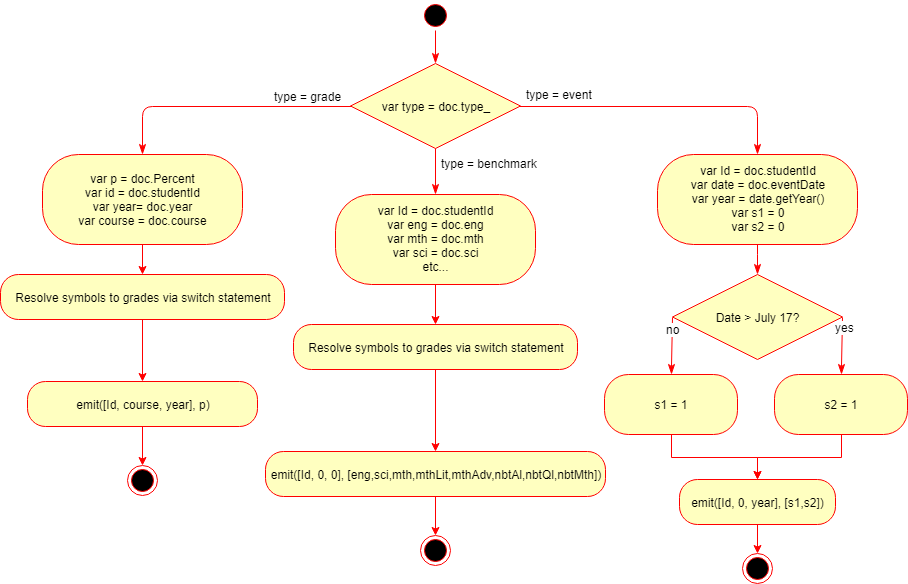
\includegraphics[scale=0.35]{./resources/figures/3-way-join-map.png}
    \end{mdframed}
    \caption[2-Way Join Map Function]{\textbf{Figure \ref{fig-3-way-join-map-function}: Map function logic required for the 2-way join.} This logic is applied to every document during index calculation (excluding documents with an \_id of ``\_design/*''). The logic used to normalize grades-as-symbols to percentages is shown in Table \ref{tbl-grades-normalize} for the Grades data, and \ref{tbl-benchmarks-normalize} for the Benchmarks data.}
    \label{fig-3-way-join-map-function}
\end{figure}

As such, during view-index retrieval it can be taken as given that for a single student ID, first documents of type Benchmark will be retrieved, followed by documents of type Event, followed by documents of type Grade.

\subsection{List Function}
\begin{figure}[H]
    \centering
    \begin{mdframed}
        \centering
        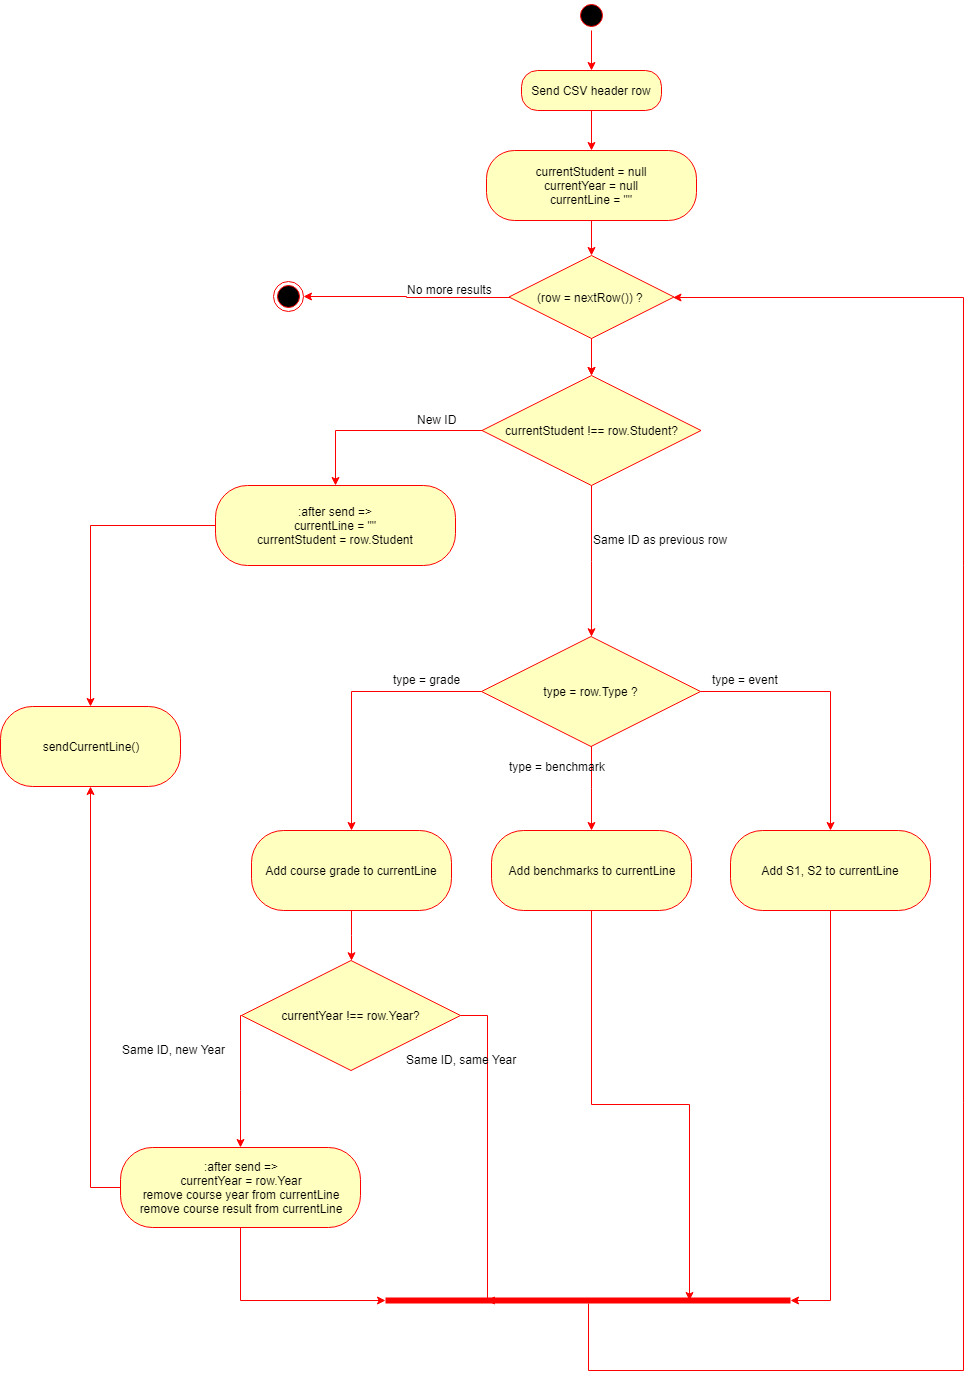
\includegraphics[scale=0.35]{./resources/figures/3-way-join-list.png}
    \end{mdframed}
    \caption[3-Way Join List Function]{\textbf{Figure \ref{fig-3-way-join-list-function}: List function logic required to join the Grades, Benchmarks and Events entities.} Activity diagram of the code executed within the callback passed to the provides function executed by CouchDB during runtime of List function.}
    \label{fig-3-way-join-list-function}
\end{figure}




















\begin{itemize}
    \item Batches of 30 000 lines are extracted iteratively (and sequentially) as an array of lines (30 000 lines per batch seemed to be the sweetspot for what could be loaded into CouchDB's \textit{\_bulk\_docs} endpoint using nETL and still receiving optimal visual feedback in terms of continuous logging)
    \item Within each batch, each line is converted to a JSON object, transforming the batch into an array of objects. These objects each have the following fields: ``event\_date'', ``event\_id'', ``uct\_id'',  ``site\_key'', ``ref''
    \item The array of objects is filtered via whitelising objects on two fields: 1) ``uct\_id'' - only IDs of students who attended CSC1015F are considered. 2) ``event\_id'' - only the value ``281'' is considered, as these are representative of `presence' events
    \item A field is added to each object in the batch (``type\_'') and give the value ``vulaEvent''
    \item Superfluous object fields are removed via a whitelisting process, resulting in a batch (an array) of objects with the fields: ``event\_date'', ``event\_id'', ``uct\_id'', ``site\_key'', ``type\_''
    \item Each batch is loaded into CouchDB using the \textit{\_bulk\_docs} endpoint (as discussed previously), and the next batch is extracted on a success message from CouchDB
\end{itemize}

\subsection*{The MapReduce function}
Compared to the function logic illustrated in \ref{result-1-map-fn}, an additional logical branch is required to handle Event data. This is shown in \ref{result-3-map-fn}.

\begin{figure}[ht]
    \centering
    \begin{mdframed}
        \centering
        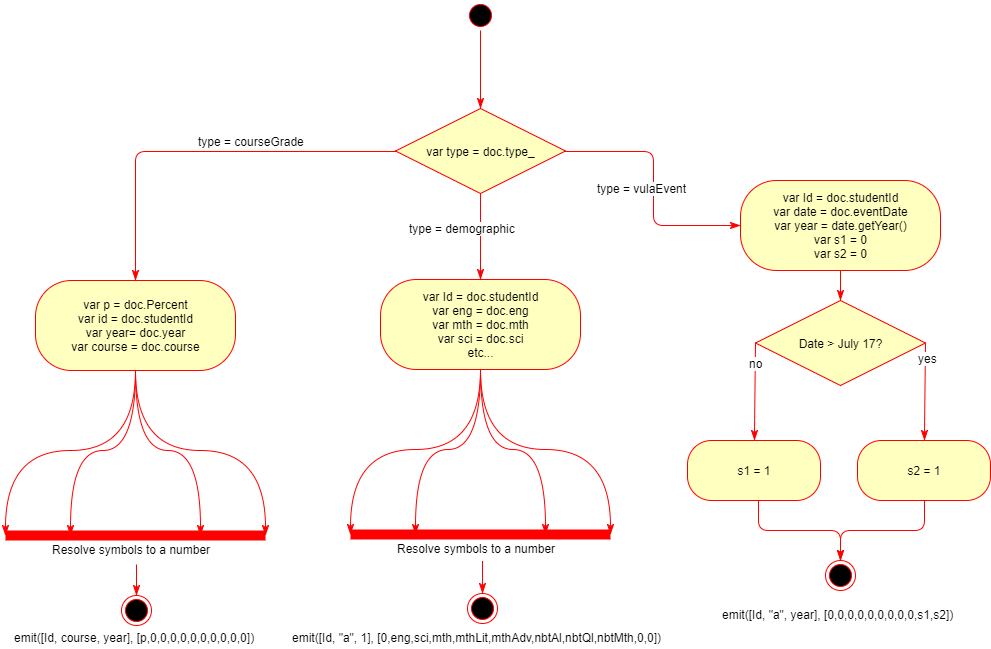
\includegraphics[scale=0.35]{./resources/figures/activity-diagram-2.png}
    \end{mdframed}
    \caption[Result 1 Map function]{\textbf{Figure \ref{result-3-map-fn}: Activity diagram showing logic Map function logic for Results 3 \& 4.} The map function comprises a decision tree with 3 logical branches depending on the type of document: FU documents are logically treated as according to the left branch, grade document the center branch, and Sakai event document as according to the logic depicted in the right hand branch. During index calculation each document is processed as according to this decision tree, with a slightly different key:value pair emitted depending on the type of document being processed - although the structure of the emitted key:value pair is identical for all document types. For documents of type 'grade', the key consists of the tuple [Id, Grade, year], the values of which are derived from the document being processed. For documents of type 'demographic', the key is a tuple that consists of the form [Id, ``a'', 2016], and for `event' documents the key emitted is of the form [Id, `a', year]. Since documents of type `event' and `demographic' do not include course information the value `a' is emitted. Similarly, for documents of type `demographic', there is no year field. So the value of `1' is always emitted. Emitting hard coded values allows for grouping documents by student Ids together and guarantees that documents of different types but with the same student Id are treated sequentially due to the nature of the b+tree storage engine. As such, aggregating different entity types across the same student Id is possible during index reading and doesn't require processing of data in addition to the retrieval process. Depending on the logical branch traversed during map function execution, different indexes of the value tuple are populated; by default this tuple instantiated on every map function execution as a list of 11 zeros. The map function then alters the value at different indexes for different document types. If the document being processed is a 'grade' document, the value at index = 0 is adjusted to be the grade percent. For 'demographic' documents, the values at indexes 1 through 8 are adjusted. And for 'event' documents, the map function adjusts values at indexes 9 and 10 before emitting the key:value pair. Since the value tuple }
    \label{result-3-map-fn}
\end{figure}

\subsection*{The List function}
Compared to the List function used to translate the index JSON output to CSV output, minor changes are implemented to handle the two additional fields in the values of the map function output. The function is included in the appendix for reference (see \ref{result-3-list})